\insertmeeting 
	{Multimedia Mayhem} 
	{09/06/22}
	{Hagerty High School}
	{Anouska, Jensen, Jorge, Karissa, Laura, Mohana, Nathan, Ritam, Robert, Samantha, Tyler}
	{Images/RobotPics/robot.jpg}
	{2:30 - 4:00}
	
\hhscommittee{General}
\noindent\hfil\rule{\textwidth}{.4pt}\hfil
\subsubsection*{Goals}
\begin{itemize}
    \item Write team bios for multimedia
    \item Start working on social media and website

\end{itemize} 

\noindent\hfil\rule{\textwidth}{.4pt}\hfil

\subsubsection*{Accomplishments}
After we got settled, we first brought our attention to the 4717 website. It hasn't been updated in a while, and with new team members, it was important we get that updated as soon as possible. While the multimedia team will be the ones to work on the website, we have a team page featuring bios of every member, so we had us all pitch in there. We spent some time typing up a bio for ourselves, which should be uploaded to the website in two weeks or so, after we take team photos. It's good to cooperate with our fellow members in multimedia, even if it's something as simple as introducing ourselves.

FTC Kickoff 2022 is coming this Saturday, so we need to get ready. We confirmed various details, such as making sure everyone is aware and everyone who is able to go is going. We sent out messages on our internal social platforms, Band and Discord, for an RSVP. We also organized for materials to be brought so we could initialize brainstorming the moment the game was revealed, and some food, for fun. This was the first event to be scheduled on a weekend, so this also serves as a low stakes test to be extra sure every member is connected and checking their socials, which will be much more important when the season actually starts.

Once our bios were finished, our multimedia people got to work setting up what they could of the website. Starting with the team page, they deleted the bios of old members, and while they didn't have the photos just yet, they included some copied photos as a template for ease of implementation later. Naturally the website wasn't in great shape to be updated, but this got them ahead of the work early, which is always a good thing.

Lastly, we rebooted our Instagram. While we had come up with ideas for it in the previous meeting, this post was just dedicated to saying we were back. Our artists of the team drew up a three-post banner in Photoshop to make for a good entry post. We're very excited to have our social media up again, and given it goes well, it will hopefully attract new sponsors and partners to work with.

Going forward, in our next meet we'll be dividing our previously planned outreach tasks, and getting everybody on Github and Onshape for collaboration in hardware and software. After that is Kickoff. Once kickoff comes around, we'll be discussing potential plans for our robot, and create a larger structured plan for the season that should carry us to victory.



% \begin{figure}[htp]
% \centering
% 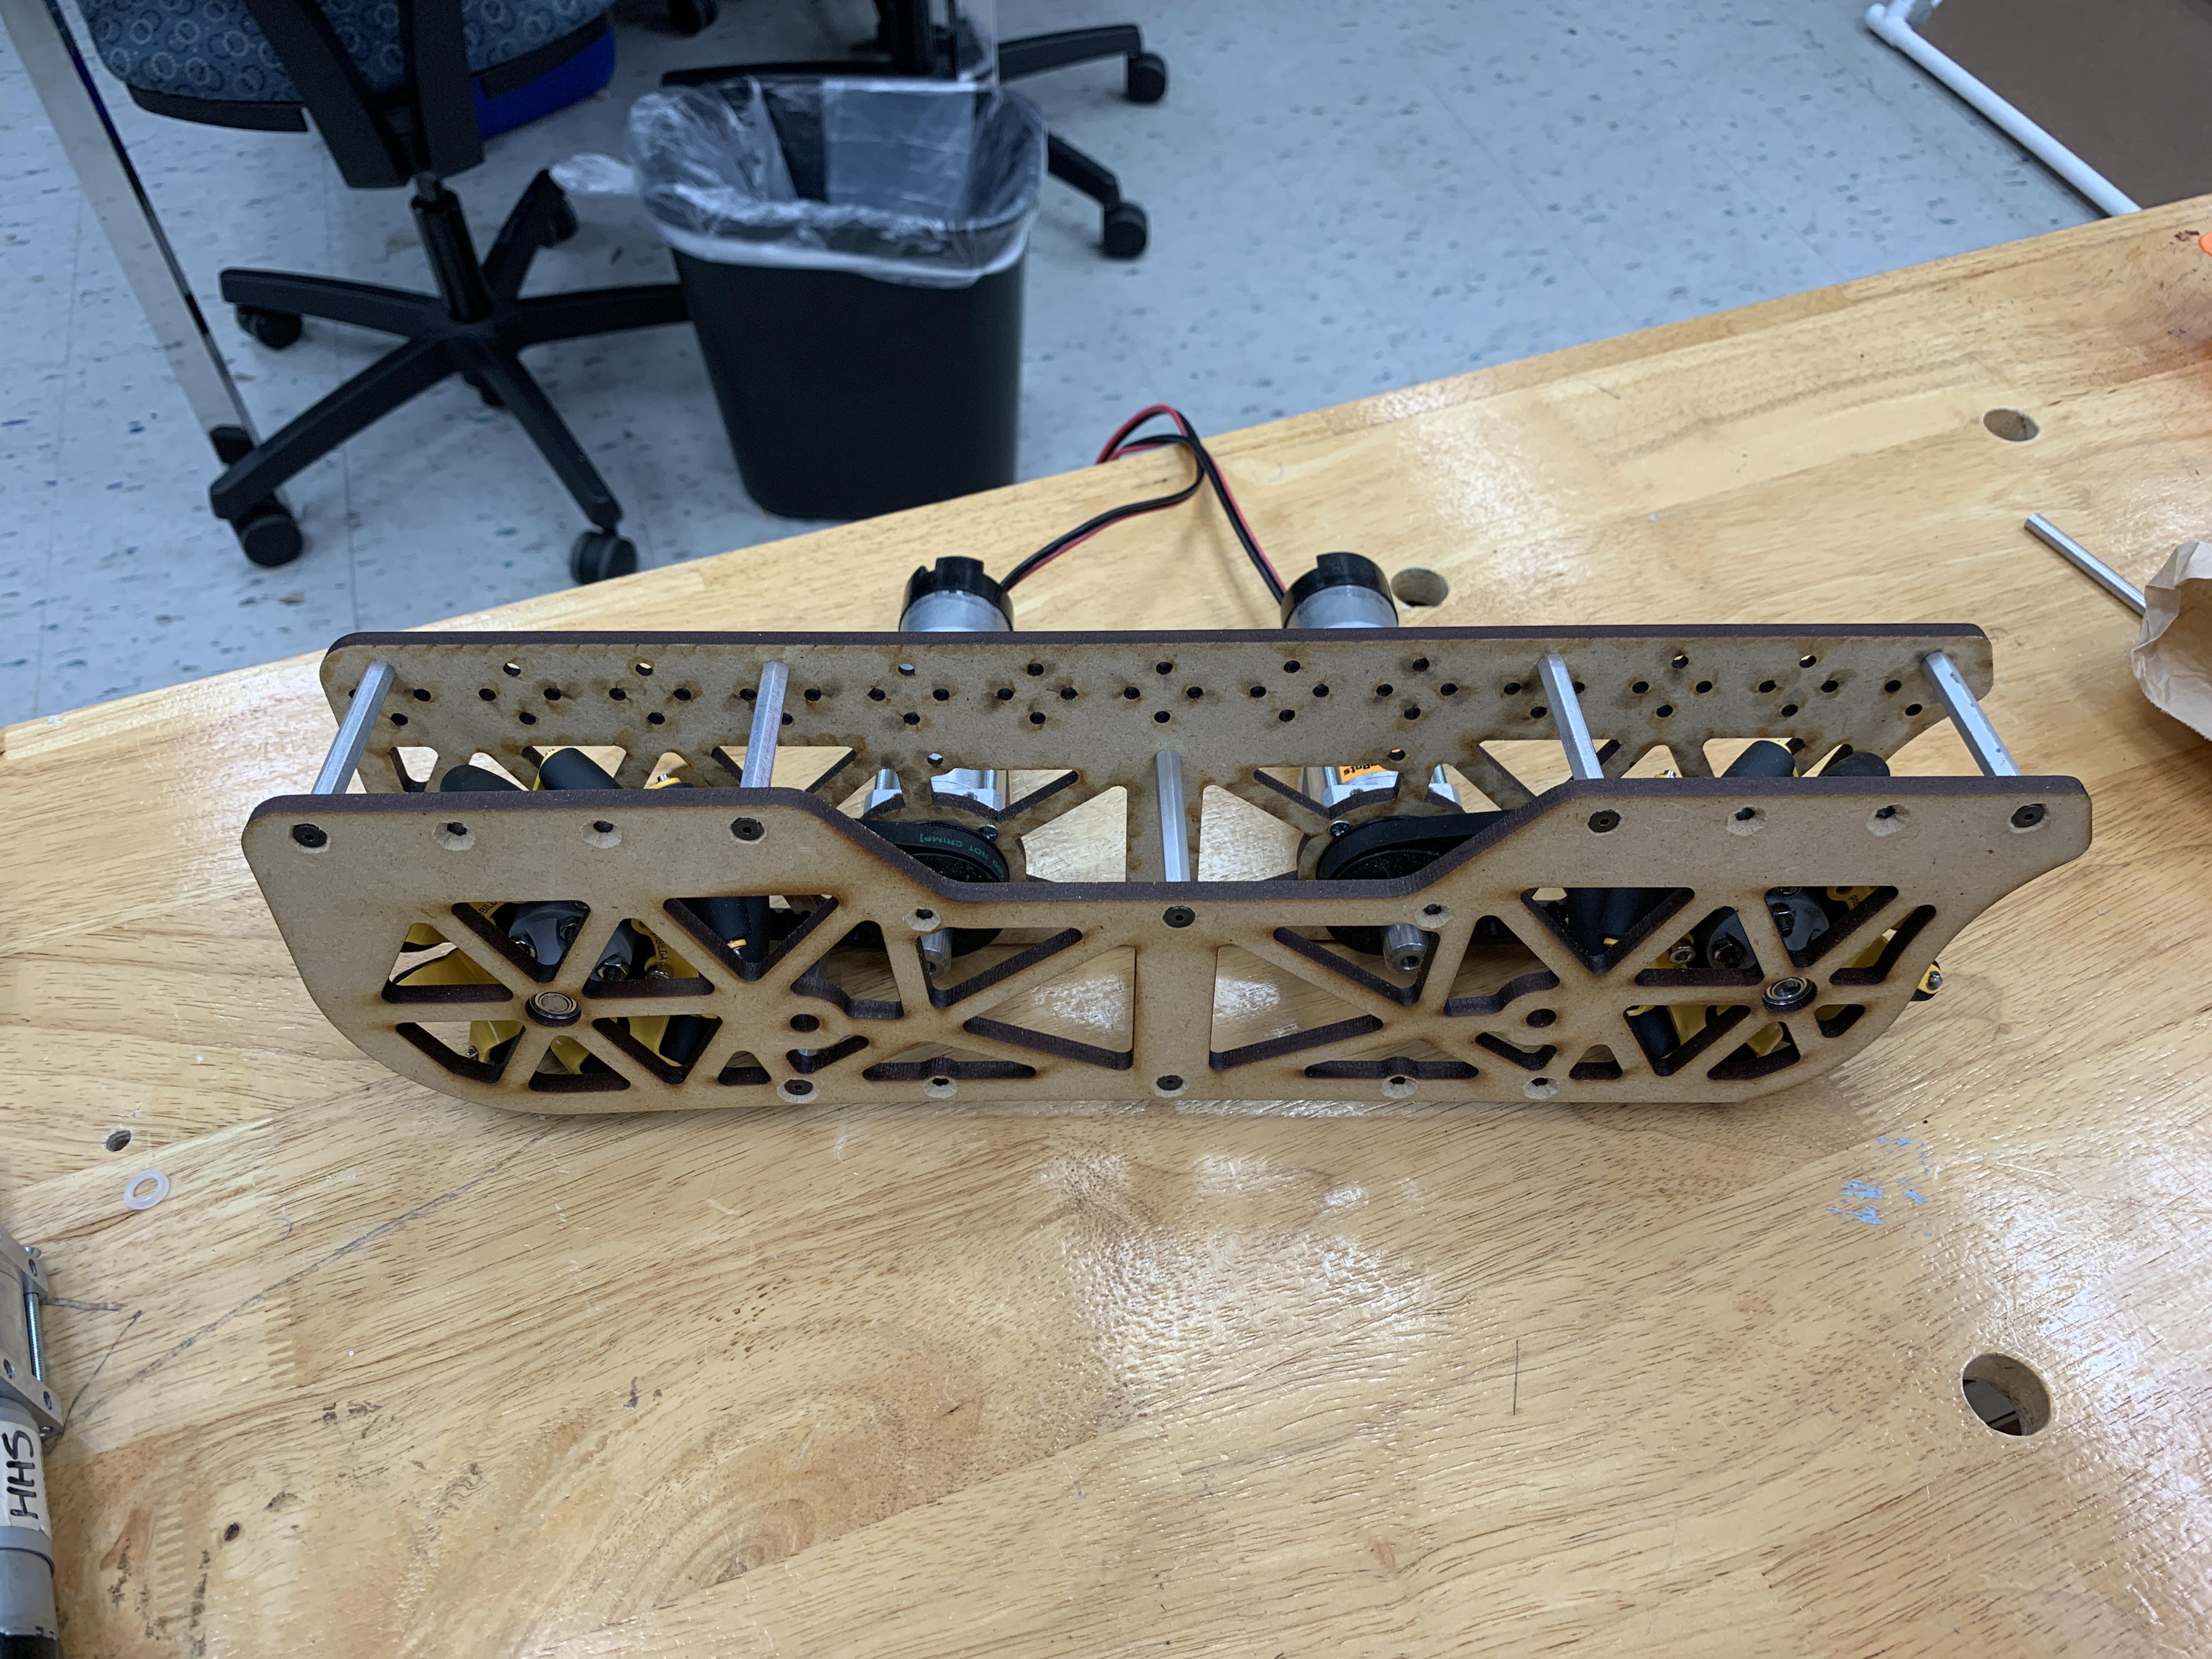
\includegraphics[width=0.9\textwidth, angle=0]{Meetings/July/07-21-21/drivetrain_7-20-21-NathanForrer.jpg}
% \caption{First half of the drivetrain.}
% \label{fig:072121_1}
% \end{figure}

\whatsnext{
\begin{itemize}
    \item Divide outreach responsibilities
	\item - Check members' access to OnShape and GitHub
\end{itemize} 
}
